
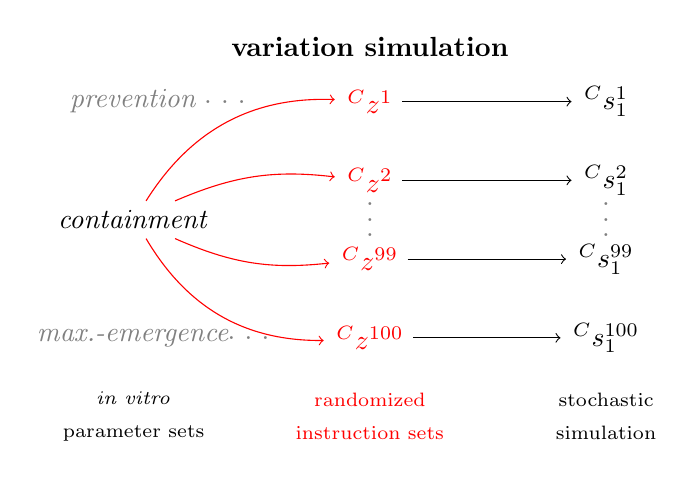
\begin{tikzpicture}[shorten >=1pt,auto]
    \node[align=center] at (3,2.2) {\textbf{variation simulation}};

  \node[]         (e1) at (0,1.5)      {\color{gray}\textit{prevention}};
  \node[]         (e2) at (0,0)      {\textit{containment}};
  \node[]         (e3) at (0,-1.5)      {\color{gray} \textit{max.-emergence}};

  \node[] (f21)  at (1.1,1.5) {\color{gray}~.~.~.};
  \node[] (f31)  at (1.4,-1.5) {\color{gray}~.~.~.};


  \node[] (d1)  at (3,1.5)  {\color{red} $\leftidx{^{C}} z ^1$};
  \node[] (d2)  at (3,0.5)  {\color{red} $\leftidx{^{C}} z ^2$};
  \node[] (d3)  at (3,-.5)  {\color{red} $\leftidx{^{C}} z ^{99}$};
  \node[] (d4)  at (3,-1.5) {\color{red} $\leftidx{^{C}} z ^{100}$};
  
  \node[] (b1)  at (6,1.5)  {$\leftidx{^{C}}s_1^{1}$};;
  \node[] (b2)  at (6,0.5)  {$\leftidx{^{C}}s_1^{2}$};;
  \node[] (b3)  at (6,-0.5) {$\leftidx{^{C}}s_1^{99}$};
  \node[] (b4)  at (6,-1.5) {$\leftidx{^{C}}s_1^{100}$};

  \node[] (f1)  at (3,0.2) {\color{gray}.};
  \node[] (f2)  at (3,0) {\color{gray}.};
  \node[] (f3)  at (3,-0.2) {\color{gray}.};
  \node[] (f1)  at (6,0.2) {\color{gray}.};
  \node[] (f2)  at (6,0) {\color{gray}.};
  \node[] (f3)  at (6,-0.2) {\color{gray}.};


  \path[->, red]  (e2)  edge   [bend left=30]  (d1);
  \path[->, red]  (e2)  edge   [bend left=15]   (d2);
  \path[->, red]  (e2)  edge   [bend right=15]  (d3);
  \path[->, red]  (e2)  edge   [bend right=30]  (d4);
  
  \path[->]  (d1)  edge                    (b1);
  \path[->]  (d2)  edge                    (b2);
  \path[->]  (d3)  edge                    (b3);
  \path[->]  (d4)  edge                    (b4);
  
  \node[align=center] at (0,-2.5) {\scriptsize \textit{in vitro} \\ \scriptsize parameter sets};
  \node[align=center] at (3,-2.5) {\scriptsize \color{red} randomized \\ \color{red} \scriptsize instruction sets};
  \node[align=center] at (6,-2.5) {\scriptsize stochastic \\\scriptsize simulation};
\end{tikzpicture}


